\documentclass[12pt]{article}
\usepackage{tikz}
\usepackage{amsthm, amsmath}
\usepackage{cite}
\usetikzlibrary{positioning}
\title{Graphz}
\author{The Graphites}
\date{\today}

\newtheorem{theorem}{Theorem}[section]
\newtheorem{lemma}[theorem]{Lemma}

\begin{document}
\maketitle
Our goal is to completely understand the cardinality of $k$-vertex-critical ($P_4 + P_1$,$H$)-free graphs when each is order 4 or higher
\begin{itemize}
\item $K_4$ - unknown
\item $diamond$ - finite ~\cite{abuadas2022vertexcritical}
\item $paw$ - finite ~\cite{abuadas2022vertexcritical}
\item $C4$ - finite ~\cite{p6c4free}
\item $claw$ - ~\cite{clawfree}
\item $P_4$ - finite since perfect
\item $\overline{K_4}$ - finite ramseys theorem
\item $P_2 + 2P_1$ - ~\cite{dichotomizing}
\item $P_3 + P_1$ - ~\cite{dichotomizing}
\item $2K_2$ - unknown
\item $K_3 + P_1$ - unknown
\end{itemize}
\begin{theorem}
hello
\end{theorem}
\begin{lemma}
there
\end{lemma}
\begin{proof}
woop woop
\end{proof}
Let $G$ be a graph. Let $S$ be the maximal independent set of $G$. The subgraph $V(G) - S$ has order $|V(G) - S|$, thus it is at most $|V(G) - S|$-colourable. The remaining vertices $S$ are 1-colourable, since they are an independent set and are not adjacent in $G$. So then our graph is at most $|V(G) - S| + 1$colourable

Let $G$ be a $k$-vertex-critical $(P_4 + P_1, 2P_2)$-free graph. Let $S$ be a maximum independent set in $G$. Let the vertices outside $S$, $V(G) - S$, be partitioned by $A$ and $B$, where $A = \{v \in V(G) - S : |N(v) \cap S = 1\}$. Then let $B = V(G) - S - A$.
Let $\forall v \in S$, $v_A = N(v) \cap A$\\
Claim 1: $\forall v,v' \in S$, $v_A$ is complete to $v'_A$\\
Proof: If $a \in v_A$ and $a' \in v'_A$ such that $a \not \sim a'$, then $\{v, v', a, a'\}$ induces a $2P_2$--- a contradiction.\\
Claim 2: $|S_A| \leq 1$\\
Proof: If $|S_A| \geq 2$, then let $v, v' \in S_A$ with $a\in v_A and a' \in v'_A$. From claim 1 we know that $a \sim a'$, so $\{v, v', a, a', x\}$ induces a $P_4 + P_1$.

For this graph to be $k$-vertex critical we can also assert that it has no comparable vertices.
Which is to say, $\forall u, v \in S$, $N(u) \not \subseteq N(v)$, or every vertex in $S$ has at least one unique neighbour compared to another vertex.\\
Let $v_1, v_2$ be two vertices in $V(G) - S$ s.t. $v_1 \sim S_A$ and $v_2 \sim $some stuff in $S_B$.
We can now assert that any element in $B$ has no neighbours in $S_A$. And that $S_A$ has no neighbours in $B$.

Let us find what happens when we look for a $(P_4 + P_1, K_3 + P_1, 2P_2)$-free graph.
Let $S$ be the maximum independent set. Let $A = \{v \in V(G) - S : |N(V) \cap S| = 1\}$
Let $B = V(G) - S - A$.
Let $S_A = \{ v \in S : N(V) \cap A \not = \emptyset \}$
Claim 3: $\forall v, v' \in S$, $v_A$ is complete to $v'_a$.
Proof: Assume $v_A \not \sim v'_A$. Then, $\{ v, v', v_A, v'_A \}$ induces a $2P_2$, a contradiction.

Claim 4: $|S_A| \leq 1 $
Proof: Assume $|S_A| \geq 2$. Then let $u, u' \in S_A$ with $a \in v_A$ and $a' \in v'_A$. From claim 1 we know that $a \sim a'$, so $\{v, v' a, a', x\}$ induces a $P_4 + P_1$ for any $x \in S - \{v, v'\}$. Note that $x$ exists, other wise the independence number of this graph is 2.
%What are the implications of this?

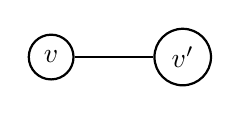
\begin{tikzpicture}[roundnode/.style={circle, draw=black, thick, minimum size = 5mm}]
\node[roundnode] (maintopic) {$v$};
\node[roundnode] (vprime) [right=of maintopic] {$v'$};

\draw[-] (maintopic.east) -- (vprime.west);
\end{tikzpicture}

Claim 5: $|A| \leq 1$
First lets make a new notation. Since $|S_A| \leq 1$, let us name that potential vertex $v_S$.
Proof: Assume $|A| \geq 2$. Then we have any two vertices in $A$ $v, v'$. From claim 4 we know that $|S_A| \leq 1$ and from claim 3 that $v$ is complete to $v'$. Since both $v, v'$ are adjacent to $v_S$, then  $\{v, v', v_S, x \}$ induces a $K_3 + P_1$, where $x \in S_B$

Once again, another claim:

There are three cases we have to work with.
For any given  $v \in B$, $v$ is either adjacent to $v_S, a,$ or both. Let's look at when $v \sim v_S$

If $v \sim v_S$, $v$ is complete to $S_B$. Proof: Assume that $v$ is not complete to $S_B$, then there exists some vertex $u \in S_B$ s.t $u \not \sim v$. we also know there is a vertexss $u' \in S_B$ that is adjacent to $v$, since $v$ is adjacent to at least 2 vertices in $S$. Then $\{v_S, a, v, u, u'\}$ induces a $P_4 + P_1$.

Claim: let there be a vertex $v'$ in $B$ s.t $v' \not \sim a$ and $v' \not \sim v_S$.

Claim: let there be a vertex $v'$ in $B$ s.t $v' \not \sim v_S$. $v'$ is not adjacent to anything in $S$ and other things.
Proof: Assume at $v'$ is adjacent to some vertex $u$ in $S_B$. Then, $\{ v', u, v_S, a \}$ induces a $2P_2$.

Some random other claim: Let $v' \not \sim v$ and $v \sim a$, then $v'$ is complete to $S$.
Proof: Assume that $v'$ is not complete to $S_B$, at least. Then, let $u$ be some vertex $\in S_B$ such that $u \sim v$ and $u \not \sim v'$. Then, $\{v_S, a, v, u, v' \}$ induces a $P_4 + P_1$. Further, if $v' \not \sim v_S$, then this leassves us with comparable vertices and thus a non-k-critical graph. Therefore, $v' \sim v_S$ and $v'$ is complete to $S$.

Let $s = S - S_B$ and $a = V(G) - B$
Let us further split $B$ into three partitions. Let $B_1 = \{v \in B : v \sim s$ and $v \not \sim a \}$ and $B_2  =\{v \in B : v \sim a$ and $v \not \sim s \}$ and finally $B_3 = \{v \in B : v \sim s$ and $v \sim a \}$.
Claim: $B_1 \cup B_3$ is complete to $S$ and $B_2$ is complete to $S - \{s\}$
$\forall s_1, s_2 \in S - \{ s \}$, $N(s_1) = B_1 \cup B_2 \cup B_3 = N(s_2)$, this makes $s_1$ and $s_2$ comparable, contradicting the criticality of the graph.
%
Now we must test the case for when $|A| = 0$. In this, we have $S$ as the maximum independent set. For this to be critical, each vertex in $S$ must have a unique neighbour such that for two vertices $s_1, s_2 \in S$, $N(s_1) \not \subset N(s_2)$ and $N(s_2) \not \subset N(s_1)$.
Let us call the set of unique neighbours $U$ and the common neighbours $C$.
Common neighbours are defined $\{ v_1, v_2 \in V - S : N(v_1) \cap S = N(v_2) \cap S \}$. Then $U = V - C$.
$\exists s_1, s_2 \in S$ s.t $\exists b \in B$ with $s_1 \sim b$ and $s_2 \sim b$.
$(N(b_1) \cap B) - \{b_2\}$ is complete to $(N(b_2) \cap B) - \{b_1\}$
Claim: $N(s_1) \cap N(s_2) \cap B = \emptyset$
$\forall b \in B - S$, $b$ has at most 1 neighbour in S, which is a contradiction of the definition of $B$.

So with this we know that $K_3$ graphs are not critical so we have to make this work with $K_3 + P_1$
With this, we can allow triangles.


Look at this claw-free graph.\\
Everytime I do it makes me laugh.\\
How did the nodes get so red\\
And where's the independent set?\\

This is what I proofed up\\
I think the logic is good enough\\
I don't how we ever went without\\
The comparable nodes lemma\\
     


Every memory of looking for $K_3$\\
I sorted all of them by criticality\\
It's hard to say it\\
Time to say it\\
It's finite, it's finite\\

HERES A DIRECTION BOIIIIS
Any graph that is $k-critical$ for $k = 5$ has a $C_5$ or a 



Here's another direction for 6-critical graphs that are $P5$ free: Any 6-critical graph that is $P_5$ free is also $P_4 + P_1 $free.

\bibliography{kritical}{}
\bibliographystyle{plain}
\end{document}